\documentclass[t,12pt]{beamer}

\mode<presentation>
\usetheme{NCSUstat}
%% \setbeamercovered{transparent}
\usepackage[english]{babel}
\usepackage[latin1]{inputenc}
\usepackage{times}
\usepackage[T1]{fontenc}
\usepackage{booktabs}
\usepackage{amsmath}
\usepackage{amssymb}
\usepackage{graphicx}
\usepackage{subfig}
\usepackage{multirow}

\graphicspath{{../images/}}

\let\bld\boldsymbol

\usepackage[backend=bibtex]{biblatex}
\bibliography{AdityaKashi-MSdefense}

% for contents slides
\AtBeginSection{
	\begin{frame}{Table of Contents}
		\tableofcontents[currentsection]
	\end{frame}
}

\title[Mesh movement and curved mesh generation] % (optional, use only with long paper titles)
{Techniques for Mesh Movement and Curved Mesh Generation}
\subtitle{for Computational Fluid Dynamics} % (optional)
\author[] % (optional, use only with lots of authors)
{Aditya Kashi}
\institute[NCSU]
{
  Department of Mechanical and Aerospace Engineering,\\
  North Carolina State University
}
\footlineupper{\insertshorttitle}
\footlinelower{\copyright{} 2016 by Aditya Kashi}
\subject{Computational Fluid Dynamics}


\date{April 27, 2016} %% uncomment to leave out the date, or to use a specific date

%%%%%%%%%%%%%%%%%%%%%%%%%%%%%%%%%%%%%%%%%%%%%%%%%%%%%%%%%%%%%%%%%%%%%%
\begin{document}

\begin{frame}
  \titlepage
\end{frame}

%%%%%%%%%%%%%%%%%%%%%%%%%%%%%%%%%%%%%%%%%%%%%%%%%%%%%%%%%%%%%%%%%%%%%%
\section{Section I : Introduction}

\subsection{Need for mesh movement}

\begin{frame}
  \frametitle{Why mesh movement?}
  \begin{block}{Mesh movement is useful in several areas of CFD}
	  \begin{itemize}
	  	\item aeroelasticity, and fluid-structure interaction in general
	  	\item shape optimization
	  	\item generation of curved meshes for spatially high-order discretizations
	  	\item others
	  \end{itemize}
  \end{block}
\end{frame}

\begin{frame}{Fluid-Structure Interaction}
	\begin{itemize}
		\item For a body-fitted grid, robust mesh-movement is required to maintain validity and quality of the mesh after imposing motion of the structural domain \footfullcite{appl:fsi}.
		\item Immersed boundary methods can also be used; both have advantages and disadvantages \footfullcite{appl:fsireview}.
	\end{itemize}
\end{frame}

\begin{frame}{Shape optimization}
	\begin{figure}
		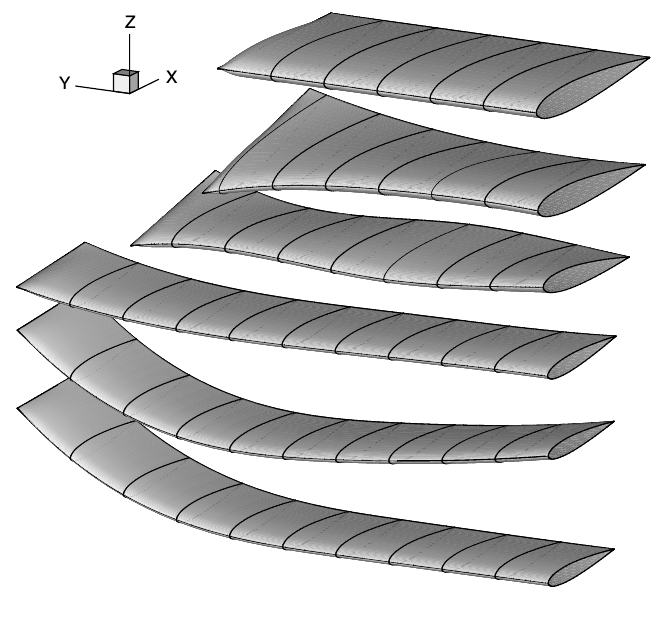
\includegraphics[scale=0.2]{ppt-illus-shapeoptimization}
		\caption{Convergence history of lift-constrained drag minimization }
	\end{figure}
	\footfullcite{appl:opt2}
\end{frame}

\subsection{Need for curved meshes}
\begin{frame}{High-order methods}
\begin{itemize}
  \item According to Wang, Fidkowski \emph{et. al.} \footfullcite{highorder}, spatially high-order methods perform better than prevailing second order methods for some kinds of simulations considering CPU time taken to achieve a given error level.
  \item One area of challenge they mention is generation of high-order meshes.
\end{itemize}
\end{frame}

\begin{frame}{The need for curved meshes}
 \begin{figure}
 	\centering
 	\subfloat{
 		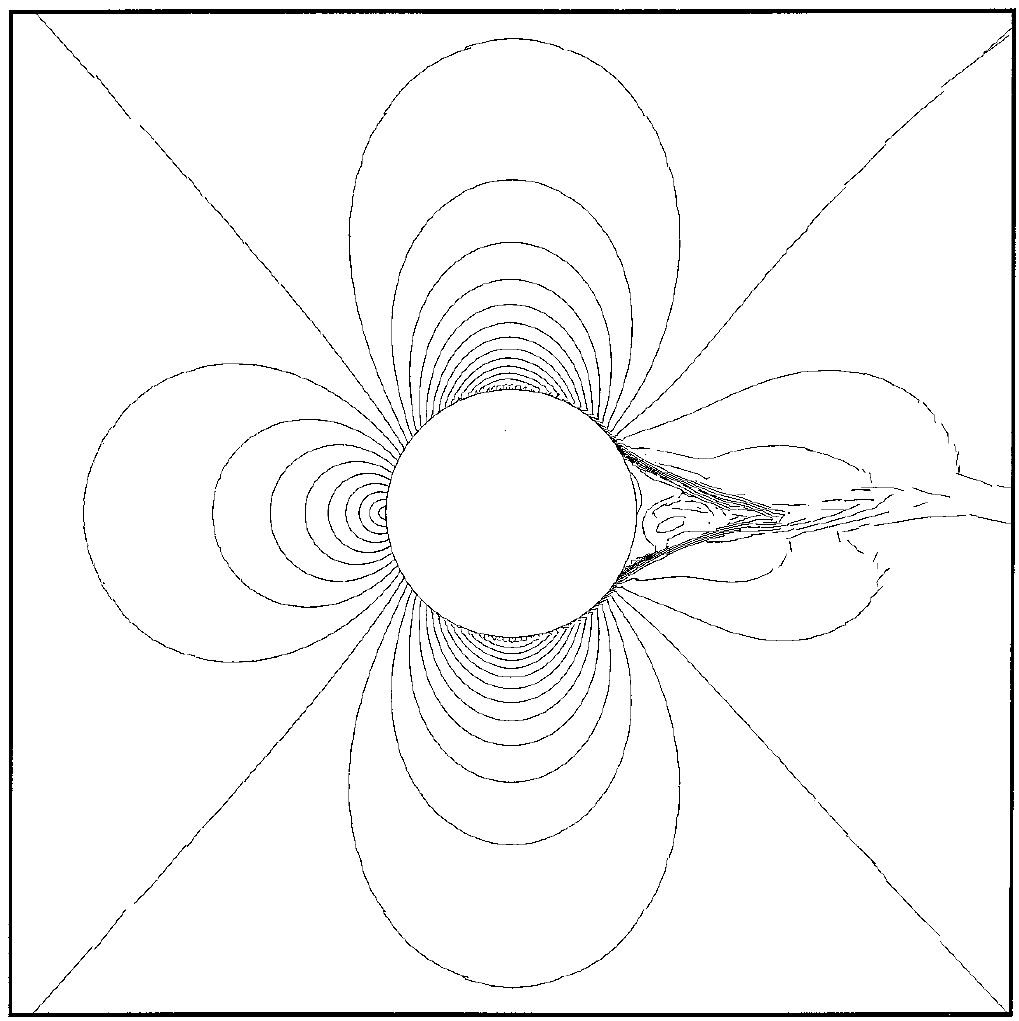
\includegraphics[scale=0.12]{bassi-linear}
 	}
 	\subfloat{
 		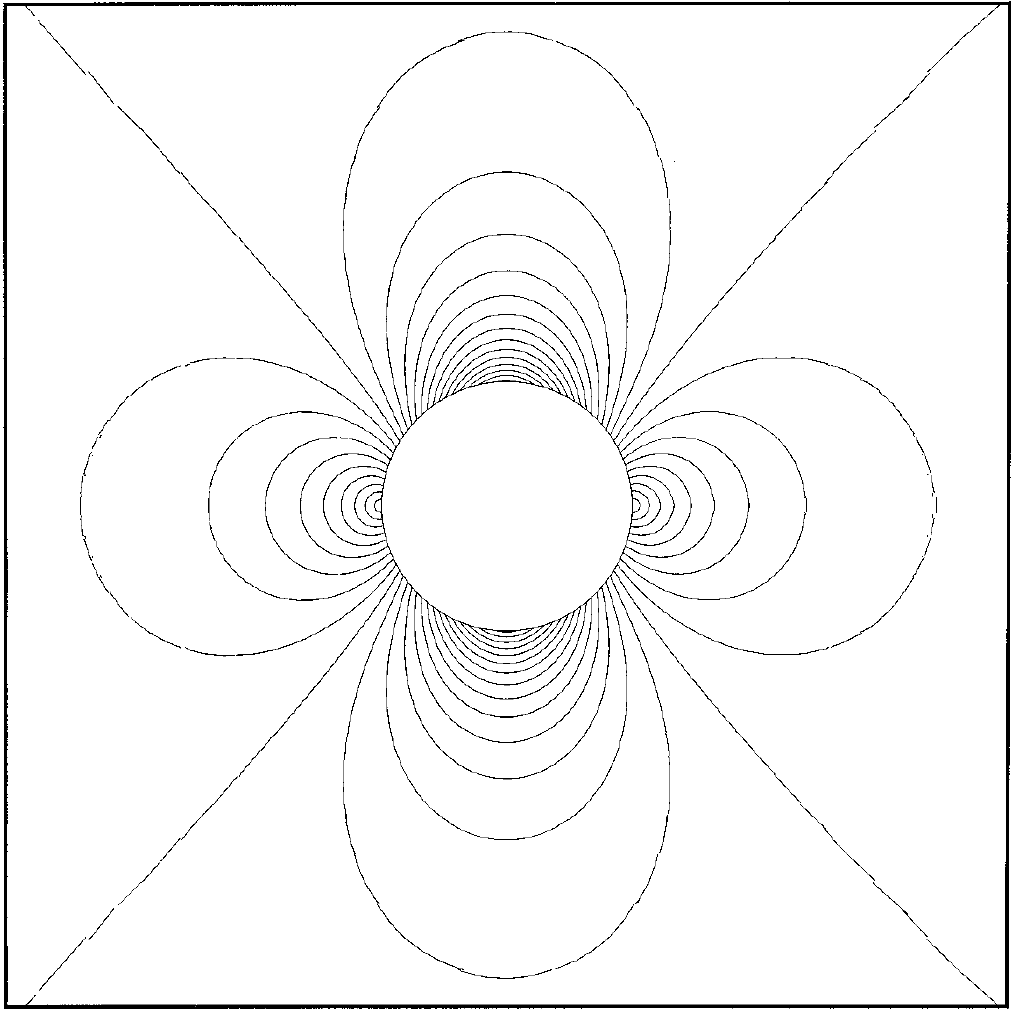
\includegraphics[scale=0.12]{bassi-q2}
 	}
 	\caption{Inviscid subsonic flow over a cylinder; left: DGP1 solution with regular linear mesh, right: DGP1 solution with quadratic (`Q2') mesh \footfullcite{appl:dgeuler}}
 	\label{fig:bassi}
 \end{figure}
\end{frame}

\begin{frame}{The need for curved meshes}
Even in less extreme cases, curved meshes are required to obtain design (p+1) order of accuracy for high-order methods such as discontinuous Galerkin methods \footfullcite{curve:geomacc}.
\end{frame}

%%%%%%%%%%%%%%%%%%%%%%%%%%%%%%%%%%%%%%%%%%%%%%%%%%%%%%%%%%%%%%%%%%%%%%
\section{Section II : Mesh movement}

\begin{frame}{Introduction}
The problem is to move the interior nodes of a mesh when a given displacement is imposed on the boundary.
\begin{itemize}
	\item At the very least: mesh elements should not get invalidated.
	\item Mesh elements should not suffer much deterioration in quality.
	\item The technique should be computationally inexpensive.
\end{itemize}
\end{frame}

\begin{frame}
Many mesh-movement methods for unstructured meshes can be found in literature. They can be broadly classified into two types.
\vspace{0.2in}
\begin{itemize}
	\item Elasticity-based methods
	\item Interpolation methods
\end{itemize}
\vspace{0.2in}
Combination of these with each other and with other techniques such as topological (connectivity) smoothing are also used \footfullcite{mm:alauzet}.
\end{frame}

\subsection{Review of methods}

\begin{frame}{Lineal spring analogy}
	Every mesh edge is treated as a linear spring in each coordinate direction \footfullcite{mm:batina}.
	 \begin{equation}
	 \sum_j k_{ij}(\Delta \mathbf{r}_i - \Delta \mathbf{r}_j) = \mathbf{0} \quad \forall i
	 \label{spring}
	 \end{equation}
	 where $i$ ranges over all nodes, $j$ ranges over points surrounding node $i$ and $\Delta \mathbf{r}_i$ is the displacement of node $i$.
	 $k_{ij}$ is the stiffness of the spring between nodes $i$ and $j$, which can be taken as
	 \begin{equation}
	 k_{ij} = \frac{1}{||\mathbf{r}_i - \mathbf{r}_j||}.
	 \end{equation}
\end{frame}
\begin{frame}{Lineal spring analogy}
	This scheme requires the solution of a (SPD) linear system of size $N_n$ (the number of mesh nodes), $n_{dim}$ (the spatial dimension of the problem) times.
\end{frame}

\begin{frame}{Torsional springs}
The lineal spring analogy fails for large deformations or stretched elements. Farhat \emph{et. al.} came up with a more robust scheme, which is also a spring analogy \footfullcite{mm:torsionsprings}.
\vspace{0.2in}
They introduce two improvements over Batina's model.
\begin{itemize}
	\item The model is closer to a structural analogy in that the displacements in each coordinate direction are coupled.
	\item `Torsional springs' are introduced at each node in each element. These are designed to prevent edges collapsing into each other due to rotational motion.
\end{itemize}
\end{frame}

\begin{frame}{Torsional springs}
The stiffness of the torsional springs at a node in an element is inversely related to the node angle in that element.
 \begin{figure}
 	\centering
 	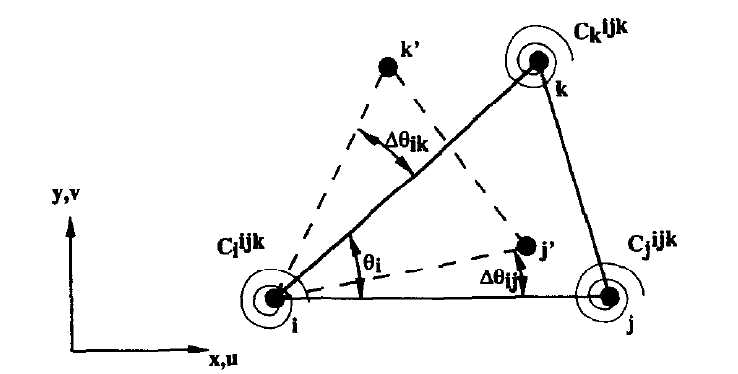
\includegraphics[scale=0.25]{torsionspring}
 	\caption{Movement of an element in torsion spring analogy}
 	\label{fig:torsion}
 \end{figure}
 A coupled SPD system of $n_{dim} N_n$ equations must be solved.
\end{frame}

\begin{frame}{Linear elasticity}
  The mesh is assumed to model a deformable solid body, which is then deformed according to the equations of solid mechanics, that is, linear or non-linear elasticity.
  
  The simplest approach is linear elasticity.
  \begin{equation}
  \nabla \cdot \bld{\sigma}  = \mathbf{0} \quad \text{in} \, \Omega
  \end{equation}
  \begin{equation}
  \bld{\sigma} = 2\mu\bld{\epsilon} + \lambda (\mathrm{tr}\boldsymbol{\epsilon}) \bld{I}
  \label{linelast:constt}
  \end{equation}
  \begin{equation}
  \bld{\epsilon} = \frac12 (\nabla\bld{u}+\nabla\bld{u}^T)
  \label{linelast:strain}
  \end{equation}
  \begin{equation}
  \bld{u} = \bld{u}_b \quad \text{on} \, \partial\Omega
  \end{equation}
\end{frame}

\begin{frame}{Stiffened Linear elasticity}
	\begin{itemize}
	\item The linear elasticity scheme is often modified by `stiffening' the mesh appropriately. 
	\item We attain some control over the propagation of deformation into the interior of the mesh, as done, for instance, by Stein \emph{et. al.} \footfullcite{mm:fsielast}.
	\item The material is stiffened based on the determinant of the local Jacobian matrix of the reference-to-physical mapping; i.e., smaller elements are stiffer than larger ones.
	\end{itemize}
\end{frame}

\begin{frame}{Nonlinear elasticity}
Claimed to be a highly robust method for mesh movement by Persson and Peraire \footfullcite{curve:persson}. 

The constitutive equation \eqref{linelast:constt} and strain-displacement relation \eqref{linelast:strain} are replaced by the `neo-Hookean' constitutive model
\begin{equation}
\bld{\sigma} = \mu ((\boldsymbol{F}^T\bld{F})\bld{F}^{-T} - \bld{F}^{-T}) + \lambda(\ln \det\bld{F})\bld{F}^{-T}
\end{equation}

Here, $\bld{F} = \frac{\partial\bld{x}}{\partial\bld{\xi}}$, $\bld{x}$ is the physical position vector of a point with coordinate $\bld{\xi}$ in the reference configuration. 

The system is solved using Newton-GMRES iterations.
\end{frame}

\begin{frame}{Elasticity-based methods}
\begin{itemize}
	\item Advantages: stiffened linear elasticity is found to be robust, and nonlinear elasticity is claimed to be very robust.
	\item Disadvantage: expensive!
	\item Also, implementation is dependent on element type and spatial dimension.
\end{itemize}
\end{frame}

\begin{frame}{Delaunay graph mapping}
 \begin{figure}
 	\centering
 	\subfloat{
 		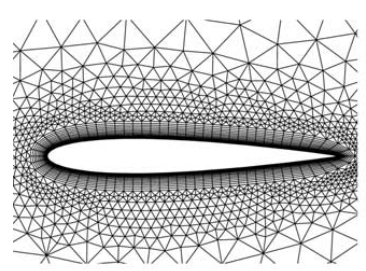
\includegraphics[scale=0.25]{dgm-mesh}
 	}
 	\subfloat{
 		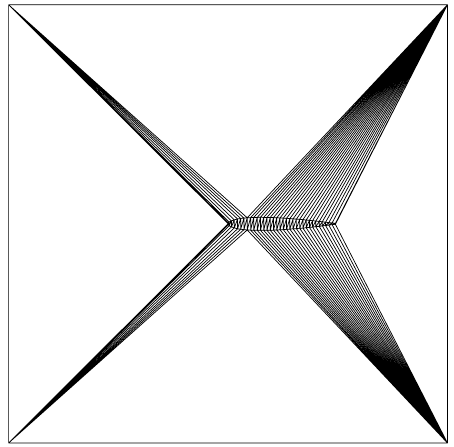
\includegraphics[scale=0.2]{dgm-dg}
 	}
 	\subfloat{
 		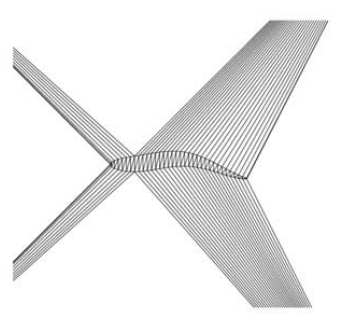
\includegraphics[scale=0.25]{dgm-moveddg}
 	}
 	\subfloat{
 		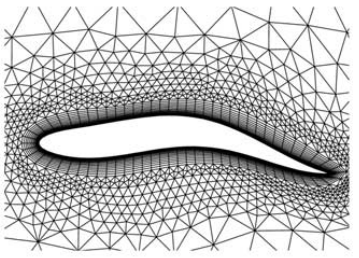
\includegraphics[scale=0.25]{dgm-movedmesh}
 	}
 	\caption{The DGM process (from left to right): original mesh, Delaunay graph, deformed Delaunay graph, deformed mesh (ref: \footfullcite{mm:dgm})}
 	\label{fig:dgmprocess}
 \end{figure}
\end{frame}

\subsection{Large rotation in inviscid mesh}

\subsection{Mesh quality}
\begin{frame}{Mesh quality metrics}
\end{frame}

\subsection{Large rotation with mesh quality}

\section{Curved mesh generation}

\section{Conclusion}

\end{document}
